\documentclass{article}
\usepackage{tikz}
\usetikzlibrary{positioning, arrows.meta, patterns}
\usepackage{subcaption}

\begin{document}

\begin{figure}
\centering
% Left Diagram: Varying Reward Function
\begin{subfigure}[b]{0.45\textwidth}
\centering
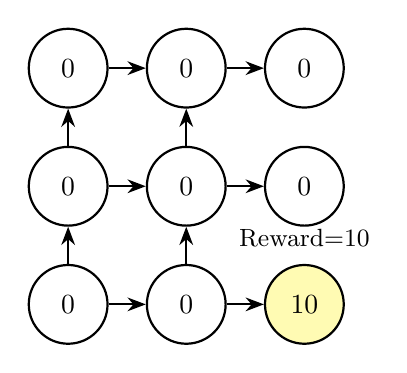
\begin{tikzpicture}[
    state/.style={circle, draw, minimum size=1cm, thick},
    reward/.style={fill=yellow!30},
    arrow/.style={-Stealth, thick}
]
    % Grid of states (3x3)
    \node[state] (s0) at (0, 0) {0};
    \node[state] (s1) at (1.5, 0) {0};
    \node[state, reward] (s2) at (3, 0) {10}; % High reward state
    \node[state] (s3) at (0, 1.5) {0};
    \node[state] (s4) at (1.5, 1.5) {0};
    \node[state] (s5) at (3, 1.5) {0};
    \node[state] (s6) at (0, 3) {0};
    \node[state] (s7) at (1.5, 3) {0};
    \node[state] (s8) at (3, 3) {0};
    
    % Arrows showing transitions (example transitions)
    \draw[arrow] (s0) -- (s1);
    \draw[arrow] (s0) -- (s3);
    \draw[arrow] (s1) -- (s2);
    \draw[arrow] (s1) -- (s4);
    \draw[arrow] (s3) -- (s4);
    \draw[arrow] (s3) -- (s6);
    \draw[arrow] (s4) -- (s5);
    \draw[arrow] (s4) -- (s7);
    \draw[arrow] (s6) -- (s7);
    \draw[arrow] (s7) -- (s8);
    
    % Highlight reward state
    \node[above=0.1cm of s2, anchor=south] {\small Reward=10};
\end{tikzpicture}
\caption{Varying reward function (highlighted state has reward 10).}
\end{subfigure}
\hfill
% Right Diagram: Varying Transition Function (Treadmill)
\begin{subfigure}[b]{0.45\textwidth}
\centering
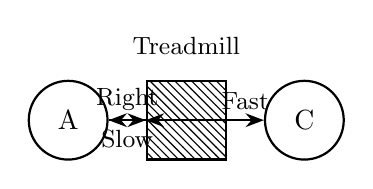
\begin{tikzpicture}[
    state/.style={circle, draw, minimum size=1cm, thick},
    treadmill/.style={rectangle, draw, thick, minimum size=1cm, pattern=north west lines},
    arrow/.style={-Stealth, thick}
]
    % States and treadmill
    \node[state] (A) at (0, 0) {A};
    \node[treadmill] (B) at (1.5, 0) {};
    \node[state] (C) at (3, 0) {C};
    
    % Treadmill arrow (leftwards)
    \draw[arrow] (B.east) -- (B.west);
    
    % Transitions
    \draw[arrow] (A) -- node[above] {\small Right} (B);
    \draw[arrow] (B) -- node[above] {\small Fast} (C);
    \draw[arrow] (B) -- node[below] {\small Slow} (A);
    
    % Labels
    \node[above=0.2cm of B, anchor=south] {\small Treadmill};
\end{tikzpicture}
\caption{Varying transition function: Treadmill pushes agent backward if slow.}
\end{subfigure}
\caption{Example MDPs with varying reward (left) and transition (right) functions.}
\end{figure}

\end{document}